\documentclass[noheader]{coursclass}

\usepackage{tikz-repère}
\usepackage{tkz-tab}
\usetikzlibrary{automata,calc,positioning}

\begin{document}

\begin{definition}[Variations d'une fonction]
	On considère une fonction $f$ définie sur un intervalle $I$.
	\begin{itemize}
		\item On dit que $f$ est \textbf{croissante} sur $I$ si pour tout réels $a$ et $b$ de $I$ tels que $a ≤ b$, on a $f(a) ≤ f(b)$.
		\item On dit que $f$ est \textbf{décroissante} sur $I$ si pour tout réels $a$ et $b$ de $I$ tels que $a ≤ b$, on a $f(a) ≥ f(b)$.
	\end{itemize}
\end{definition}

\begin{exemple}
	\directlua{
		function draw_path(f, a, b)
		tex.print("\\draw[thick,red,dashed] (", a, ",0) node[below] {$a$} -- (", a, ",", f(a), ") -- (0,", f(a), ") node[left] {$f(a)$};")
		tex.print("\\draw[thick,red,dashed] (", b, ",0) node[below] {$b$} -- (", b, ",", f(b), ") -- (0,", f(b), ") node[left] {$f(b)$};")
		end
	}
	\begin{minipage}{0.45\textwidth}
		\begin{center}
			\begin{tikzpicture}[scale=0.7]
				\tikzRepere{-1}{3}{-1}{3}[][]
				\draw[thick,blue,domain=-1:3] plot({\x},{exp(\x - 2)});
				\directlua{draw_path(function (x) return math.exp(x - 2) end, 1.5, 2.5)}
			\end{tikzpicture}

			On a $a ≤ b$, et $f(a) ≤ f(b)$,

			donc $f$ est croissante.
		\end{center}
	\end{minipage}\hspace{0.05\textwidth}
	\begin{minipage}{0.45\textwidth}
		\begin{center}
			\begin{tikzpicture}[scale=0.7]
				\tikzRepere{-1}{3}{-1}{3}[][]
				\draw[thick,blue,domain=-1:3] plot({\x},{-exp(\x - 2) + 2});
				\directlua{draw_path(function (x) return -math.exp(x-2)+2 end, 1, 2.2)}
			\end{tikzpicture}

			On a $a ≤ b$, et $f(a) ≥ f(b)$,

			donc $f$ est décroissante.
		\end{center}
	\end{minipage}
\end{exemple}

\vfill

\begin{greybox}[frametitle={Tableau de variations}]
	Un \textbf{tableau de variations} résume les intervalles sur lesquelles la fonction est croissante ou décroissante :

	\begin{minipage}{0.45\textwidth}
		\begin{center}
			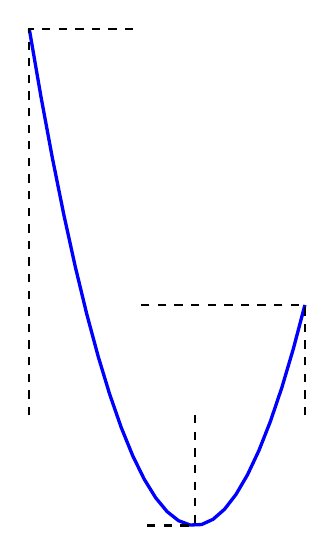
\begin{tikzpicture}[scale=0.7]
				\tikzRepere{-3}{3}{-2}{7}
				\draw[very thick,blue,domain=-2:3] plot({\x},{\x*\x - 2*\x - 1});
				\foreach \x/\y in {-2/7,1/-2,3/2} {
						\draw[thick,dashed] (\x,0) -- ++(0,\y) -- (0,\y);
					}
			\end{tikzpicture}
		\end{center}
	\end{minipage}\hspace{0.05\textwidth}
	\begin{minipage}{0.45\textwidth}
		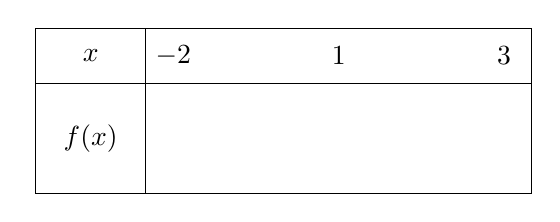
\begin{tikzpicture}[scale=0.7]
			\tkzTabInit{$x$ / 1 , $f(x)$ / 2}{$-2$, $1$, $3$}
			\tkzTabVar{}
		\end{tikzpicture}
	\end{minipage}
\end{greybox}

\end{document}
